% \vspace{-3mm}
\section{Method}
% \vspace{-2mm}

We consider the problem of synchronized action-conditioned multi-agent video generation. Formally, the goal is to learn a function $\gamma\text{-World}(\{o_{1:t}^p\}_{p=1}^P,\, \{a_{1:t}^p\}_{p=1}^P)$, that takes a sequence of past observations and actions for $P$ agents as input and produces the next observation for each agent $\{o_{t+1}^p\}_{p=1}^P$. Because we focus on the multi-agent setting, it is important to note that $\{o_t^p\}_{p=1}^P$ correspond to different perspectives of the same underlying world state at time $t$.

Our proposed model builds on transformer-based latent video diffusion models adapted for autoregressive generation, in which rotary position embeddings encode spatial and temporal locations (\S\ref{sec:preliminaries}). We modify this position embedding to account for agent identities and propose a multi-agent aware attention masking mechanism to reduce computational cost (\S\ref{sec:simplex-rotary-agent-encoding}). Finally, the full model is trained in two steps: first, a bidirectional teacher model is trained, and then it is distilled into a causal student model that supports the streaming setting (\S\ref{sec:causal-distillation}). An overview of the method is provided in figure~\ref{fig:method}.

\begin{figure*}[t]
  \centering
  % \vspace{-10mm}
  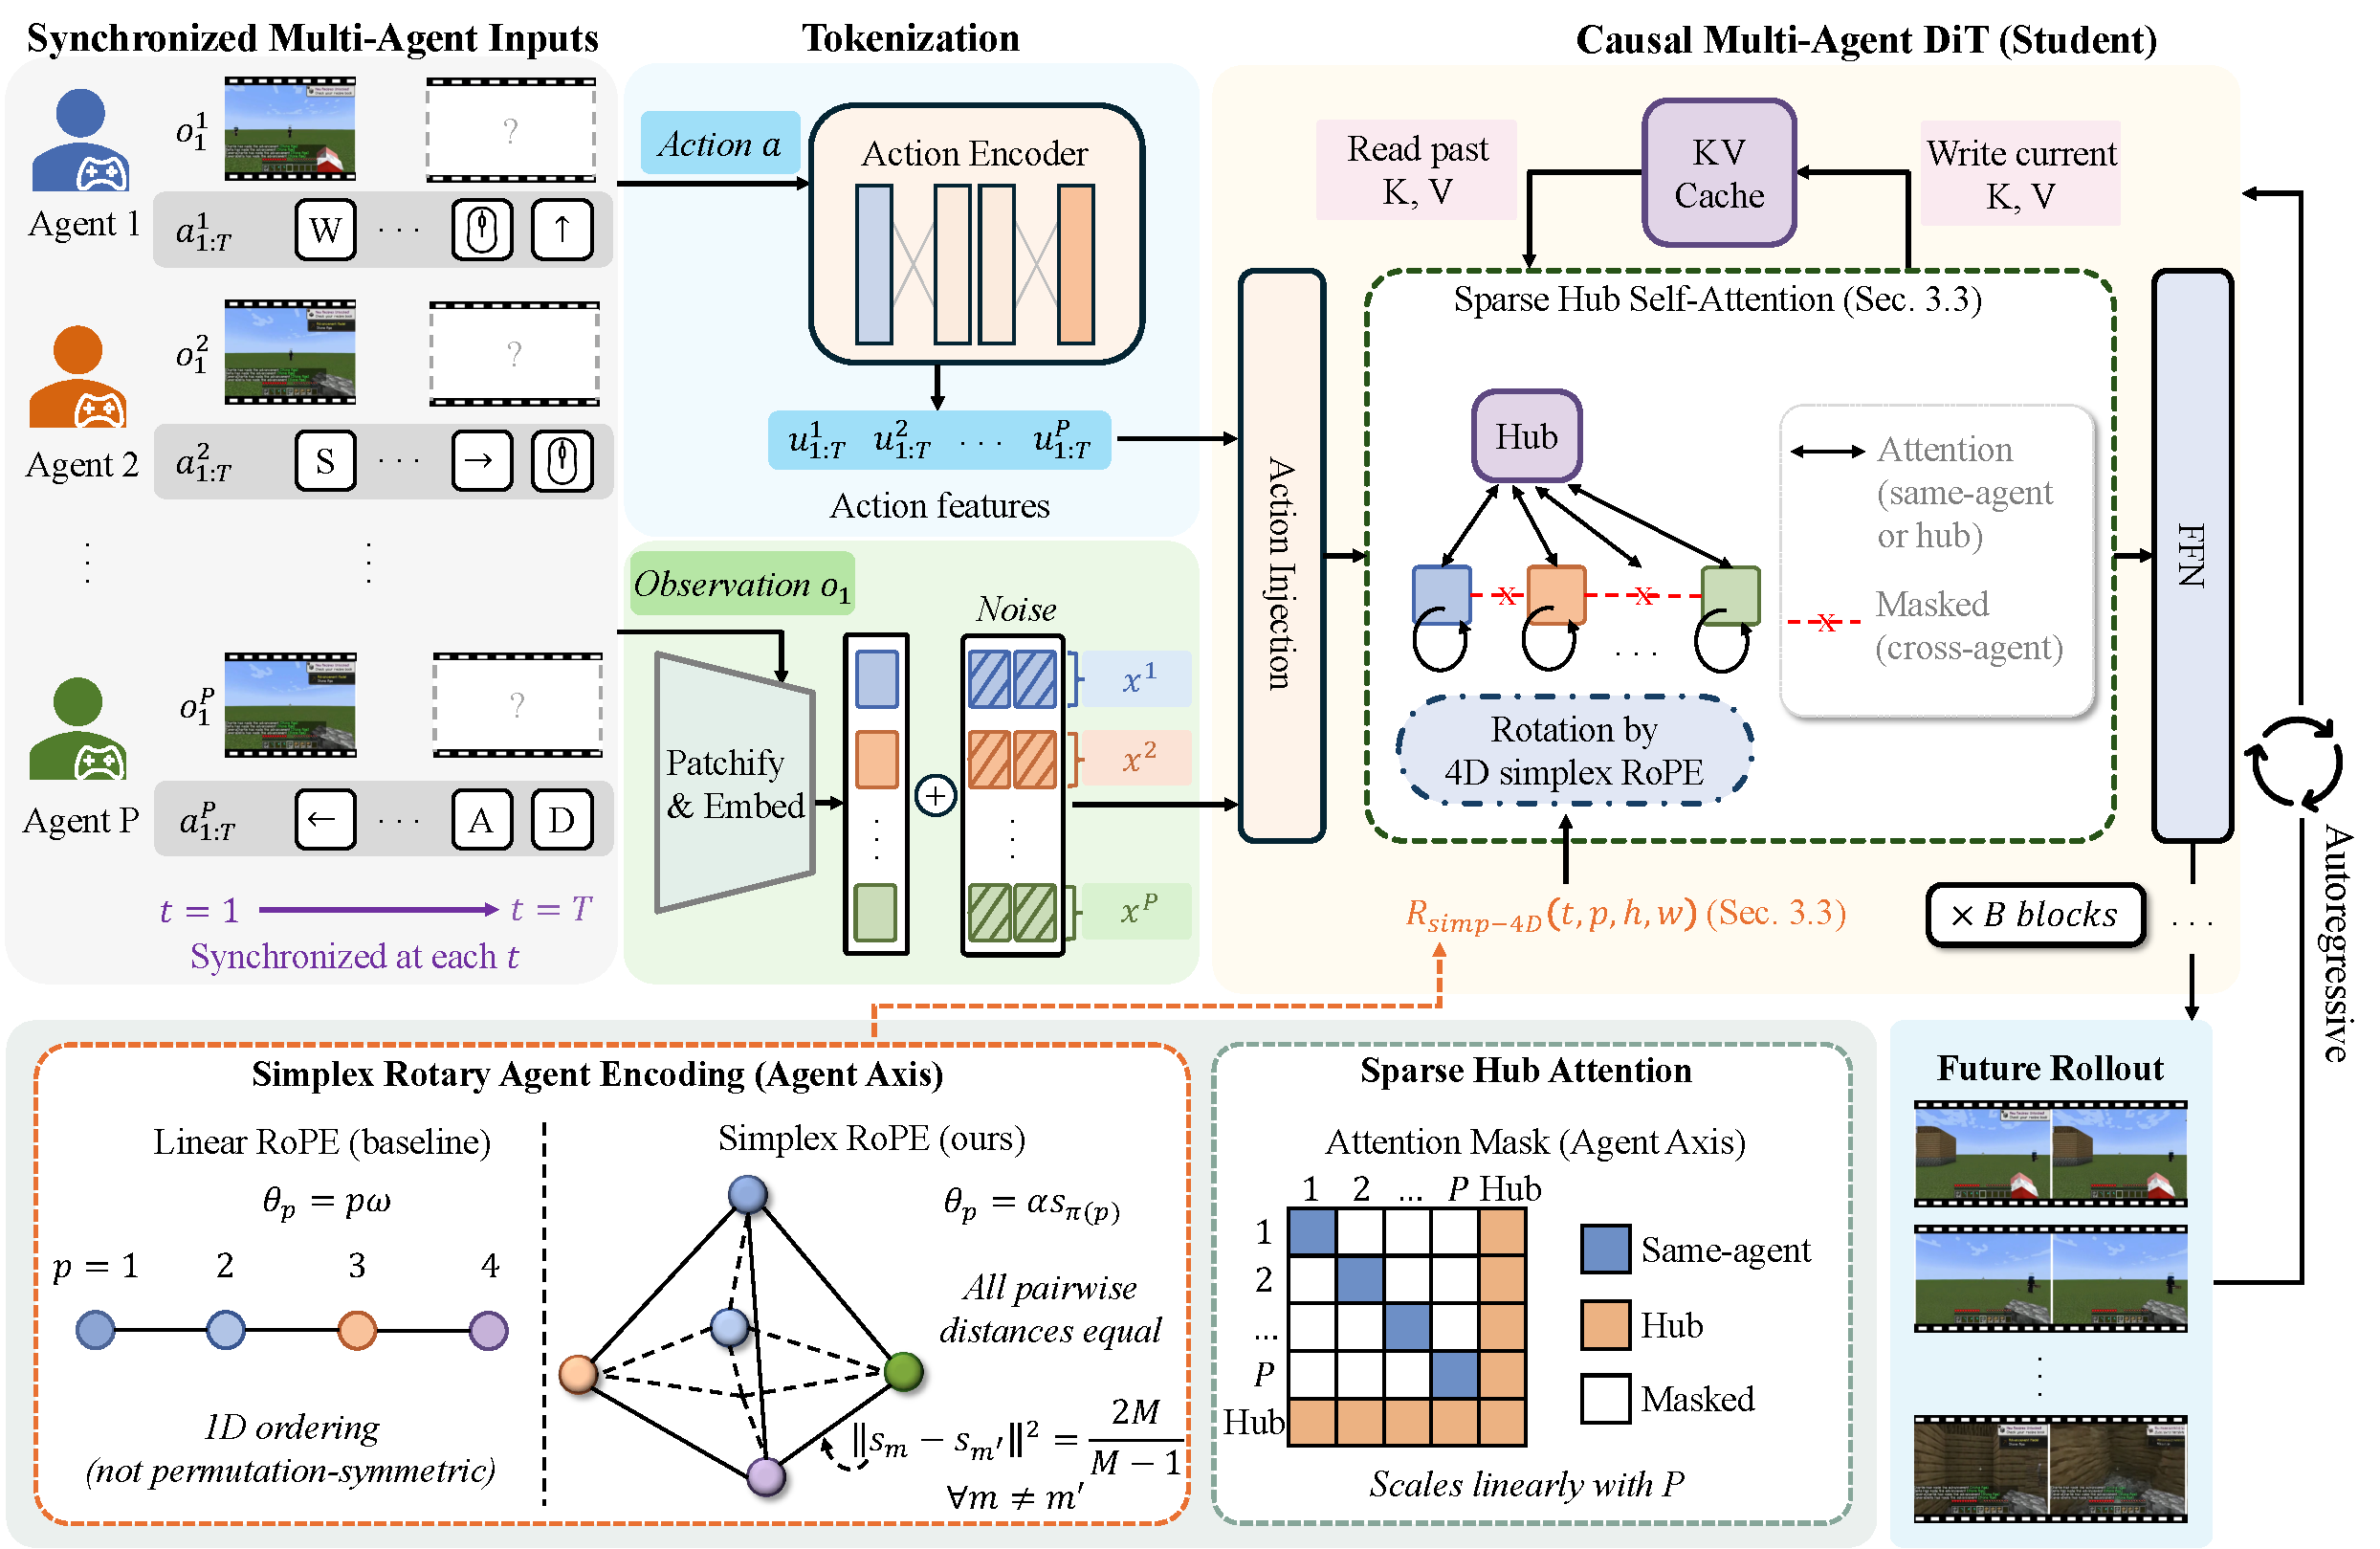
\includegraphics[width=\linewidth]{figures/multiagent_method.pdf}
  \caption{\textbf{Method overview.}
  \ours takes synchronized observations and actions from multiple agents as input, tokenizes each agent stream with shared visual and action encoders, and generates future multi-agent rollouts with a causal multi-agent DiT.
  We formulate the input with an explicit synchronized agent axis, encode exchangeable agent identity using Simplex Rotary Agent Encoding (\S\ref{sec:simplex-rotary-agent-encoding}), and route cross-agent information through Sparse Hub Attention (\S\ref{sec:sparse-hub-attention}).
  During streaming inference, the causal student uses KV caches for past visual tokens and hub states to preserve block-causal generation while scaling efficiently with the number of agents (\S\ref{sec:causal-distillation}).}
  % \vspace{-4mm}
  \label{fig:method}
\end{figure*}



\subsection{Preliminaries}
\label{sec:preliminaries}
% \vspace{-2mm}

\noindent\textbf{Latent video diffusion.}
We build on DiT-based latent video diffusion transformers~\cite{peebles2023scalable,wan}.
Let $\mathbf{z}_0\in\mathbb{R}^{T\times H\times W\times C_z}$ denote a clean video latent with $T$ temporal positions, $H\times W$ spatial positions, and $C_z$ channels per token.
We adopt the flow-matching objective~\cite{lipman2022flow}: given $\mathbf{z}_0$, a noise sample $\boldsymbol{\epsilon}\sim\mathcal{N}(\mathbf{0},\mathbf{I})$, and a noise level $\sigma\in[0,1]$, we form the linear interpolant
\begin{equation}
\mathbf{z}_{\sigma}=(1-\sigma)\,\mathbf{z}_0+\sigma\,\boldsymbol{\epsilon},
\end{equation}
and train a velocity field $v_\theta$ to regress its time derivative $\boldsymbol{\epsilon}-\mathbf{z}_0$:
\begin{equation}
\mathcal{L}_{\mathrm{FM}}
=
\mathbb{E}_{\mathbf{z}_0,\,\boldsymbol{\epsilon},\,\sigma}\!\left[
\left\|v_{\theta}(\mathbf{z}_{\sigma},\sigma,\mathcal{C})-(\boldsymbol{\epsilon}-\mathbf{z}_0)\right\|_2^2
\right],
\end{equation}
where $\mathcal{C}$ denotes conditioning signals such as initial observations and agent actions.


\noindent\textbf{Causal autoregressive video generation.}
Standard video diffusion transformers are typically bidirectional: during denoising, tokens can attend to the full latent video, which improves global consistency but prevents streaming rollout.
To enable autoregressive generation, Self-Forcing~\cite{huang2025self} combines Diffusion Forcing~\cite{chen2024diffusion} with block-causal attention.
The latent sequence is partitioned into temporal blocks of $n$ frames, an independent noise level $\sigma_b\sim\mathcal{U}(0,1)$ is sampled for each block, and each query attends only to keys from the same or earlier blocks.
Attention remains bidirectional within each block, matching streaming inference where the model repeatedly denoises the current block conditioned on previously generated blocks.

\noindent\textbf{Rotary Position Embedding (RoPE).}
Video diffusion transformers commonly use 3D RoPE~\cite{rope} to inject relative position into self-attention by rotating query and key features along factorized temporal and spatial axes.
The rotary head dimensions are split into temporal, height, and width bands of sizes $d_t,d_h,d_w$, with $d_t+d_h+d_w=d_{\mathrm{rope}}$.
For a token at coordinate $(t,h,w)$, the 3D RoPE operator is
\begin{equation}
\mathbf{R}_{\mathrm{3D}}(t,h,w)
=
\mathrm{diag}\!\left(\mathbf{R}_{t}(t),\,\mathbf{R}_{h}(h),\,\mathbf{R}_{w}(w)\right),
\end{equation}
where each $\mathbf{R}_x(x)$ is a block-diagonal of 2D rotations whose angles follow the standard RoPE frequency schedule~\cite{rope}.

% \vspace{-2mm}
%\subsection{Problem Formulation}
%\label{sec:multi-agent-formulation}
% \vspace{-2mm}


%We consider $P$ synchronized agents acting in a shared environment over $T$ latent frames.
%At each time $t$, agent $p$ receives an observation $o_t^p$ and executes an action $a_t^p$.
%The observations from all agents are synchronized: $\{o_t^p\}_{p=1}^P$ correspond to different perspectives of the same underlying world state at time $t$, and the joint action $\{a_t^p\}_{p=1}^P$ drives the subsequent world evolution.

\subsection{Model Design}
\label{sec:model-design}

Our model starts by performing visual tokenization, after which a clean multi-agent latent is represented as
$\mathbf{Z}_0\in\mathbb{R}^{P\times T\times H\times W\times C_z}$,
which extends the single-agent latent $\mathbf{z}_0$ from \S\ref{sec:preliminaries} with an explicit agent axis indexed by $p\in\{1,\ldots,P\}$.
The model is conditioned on initial observations and per-agent action sequences, and predicts future latent observations for all agents jointly.
This formulation encourages generated rollouts to remain consistent across both time and agent perspectives.
At inference, the first observations $\{o_1^p\}_{p=1}^P$ are encoded as context, while future latent tokens are initialized from noise and denoised block by block under the per-agent action sequences.


\noindent\textbf{Action conditioning.}
\label{sec:action-conditioning}
Each agent is controlled by its own action sequence $\mathbf{a}^p_{1:T}$.
We use a shared action encoder $f_a$ across all agents to map each action to a hidden action feature
$\mathbf{u}_t^p = f_a(a_t^p) \in \mathbb{R}^{D}$,
where $D$ is the DiT hidden dimension.
For discrete or multi-component controls, we embed each action component and combine the embeddings with a lightweight MLP.

Let $\mathbf{x}_{\ell,p,t,h,w}\in\mathbb{R}^{D}$ denote the transformer state at layer $\ell$ for agent $p$, frame $t$, and spatial position $(h,w)$.
At transformer block $\ell$, the action feature is projected to a layer-specific action bias
\begin{equation}
\boldsymbol{\beta}_{\ell,t}^p = g_\ell(\mathbf{u}_t^p) \in \mathbb{R}^{D},
\end{equation}
and broadcast to all spatial tokens of the corresponding agent and frame:
\begin{equation}
\mathbf{x}_{\ell,p,t,h,w}
\leftarrow
\mathbf{x}_{\ell,p,t,h,w}
+
\boldsymbol{\beta}_{\ell,t}^p .
\end{equation}
The biased tokens are then passed to self-attention.
The action encoder and projection layers are shared across agents, so the same action has the same representation regardless of agent identity. 



\noindent\textbf{Simplex Rotary Agent Encoding.}
\label{sec:simplex-rotary-agent-encoding}
To distinguish agents without imposing an arbitrary slot ordering, we extend the 3D RoPE coordinate from \S\ref{sec:preliminaries} with an explicit agent axis $p$.
We partition the rotary head dimension as
$d_{\mathrm{rope}}=d_t+d_p+d_h+d_w$,
which yields the 4D rotary operator
\begin{equation}
\mathbf{R}_{\mathrm{4D}}(t,p,h,w) = \mathrm{diag}\!\left(\mathbf{R}_{t}(t),\,\mathbf{R}_{p}(p),\,\mathbf{R}_{h}(h),\,\mathbf{R}_{w}(w)\right).
\end{equation}
A natural instantiation of $\mathbf{R}_{p}$ is to assign each agent a scalar phase $\boldsymbol{\theta}_p=p\,\boldsymbol{\omega}$ for some frequency vector $\boldsymbol{\omega}$.
However, this places exchangeable agents on a one-dimensional line: different pairs receive different rotary distances depending on $|p-q|$, and the indexing convention can make certain slots structurally special.
Learned per-slot embeddings have a different failure mode: they tie agent identity to a fixed roster and break permutation symmetry.
We instead seek an encoding that distinguishes agents while making all agent identities \emph{equidistant and exchangeable}.


To achieve this, we represent agents as vertices of a regular simplex in rotary angle space.
Let $V$ denote a fixed simplex pool size chosen at training time, corresponding to the maximum number of supported agent identities, with $V\leq d_p/2+1$.
We construct $V$ simplex vertices in the $d_p/2$-dimensional agent-angle space:
\begin{equation}
\mathbf{s}_v
=
\sqrt{\tfrac{V}{V-1}}\;
\mathbf{Q}\!\left(\mathbf{e}_v-\tfrac{1}{V}\mathbf{1}\right)
\in\mathbb{R}^{d_p/2},
\qquad v=1,\ldots,V,
\end{equation}
where $\mathbf{e}_v\in\mathbb{R}^{V}$ is the $v$-th one-hot vector, $\mathbf{1}\in\mathbb{R}^{V}$ is the all-ones vector, and $\mathbf{Q}$ is a linear isometry from the zero-mean subspace of $\mathbb{R}^{V}$ into $\mathbb{R}^{d_p/2}$.


The resulting vertices have unit norm and equal pairwise distance:
\begin{equation}
\|\mathbf{s}_v\|_2=1,\qquad
\|\mathbf{s}_v-\mathbf{s}_{v'}\|_2^2=\tfrac{2V}{V-1}
\quad\text{for all }v\neq v',
\end{equation}
with the proof given in Appendix~\ref{app:simplex-equidistance}.


For a batch with $P\leq V$ active agents, we sample an injective assignment
$\pi:\{1,\ldots,P\}\rightarrow\{1,\ldots,V\}$
and assign agent $p$ to simplex vertex $\mathbf{s}_{\pi(p)}$.
The agent-band rotation angles are
\begin{equation}
\boldsymbol{\theta}_p=\alpha\,\mathbf{s}_{\pi(p)},
\end{equation}
where $\alpha>0$ controls the strength of agent separation.
Replacing $\mathbf{R}_{p}$ with the corresponding simplex rotation $\mathbf{R}_{\mathrm{simp}}(\pi(p))$ gives
\begin{equation}
\mathbf{R}_{\mathrm{simp\text{-}4D}}(t,p,h,w)
=
\mathrm{diag}\!\left(
\mathbf{R}_{t}(t),
\mathbf{R}_{\mathrm{simp}}(\pi(p)),
\mathbf{R}_{h}(h),
\mathbf{R}_{w}(w)
\right).
\end{equation}

This encoding is parameter-free, permutation-symmetric, and does not introduce learned per-slot identities.
The simplex pool provides a direct mechanism for agent-count scaling.
During training, active agents are randomly assigned to distinct vertices from the fixed pool, discouraging slot-specific overfitting.
At inference, additional agents can be activated by selecting additional unused vertices from the same pool, without changing the transformer architecture or introducing new learned identities.
For pretrained video DiTs that lack an explicit agent band, we follow ReRoPE~\cite{li2026rerope} and allocate $d_p$ dimensions from the low-frequency end of the temporal band, leaving the high-frequency temporal and spatial bands intact.



\noindent\textbf{Sparse Hub Attention.}
\label{sec:sparse-hub-attention}
A direct way to model cross-agent interaction is dense joint attention over all agent tokens, as in Solaris~\cite{savva2026solaris}.
With $L=HW$ tokens per frame and $P$ agents, dense cross-agent attention over a block of $n$ frames costs $\mathcal{O}(P^2n^2L^2)$.
This becomes expensive as the number of agents grows, and it is often unnecessary: in many shared-world settings, agents influence one another primarily through a compact evolving environment state rather than through dense token-level pairwise exchange at every layer.

We therefore introduce \emph{Sparse Hub Attention} (SHA), a hub-mediated attention topology that adds a small set of learnable hub tokens as a compact shared communication state.
Agent tokens attend only to tokens from the same agent stream and to the hub tokens.
Hub tokens attend to all agents and to other hub tokens.
Direct attention between distinct agent streams is masked, so cross-agent information flows through a two-hop path: agent~$\rightarrow$~hub~$\rightarrow$~agent.


We organize the sequence as $PTL$ agent tokens followed by $TK$ hub tokens, with $K$ hub tokens per latent frame.
The hub tokens are drawn from a learnable matrix $\mathbf{H}\in\mathbb{R}^{K\times D}$, broadcast across frames, and removed from the output, so they act purely as internal communication states.
Let $\rho(i)\in\{1,\ldots,P,\mathrm{hub}\}$ denote the identity of token $i$.
The hub-and-spoke topology is defined by
\begin{equation}
\mathcal{M}_{\mathrm{hub}}(i,j)
=
\mathbf{1}\!\left[
\rho(i)=\rho(j)
\;\vee\;
\rho(i)=\mathrm{hub}
\;\vee\;
\rho(j)=\mathrm{hub}
\right].
\end{equation}
For causal autoregressive generation, we compose this topology with the block-causal mask (\S\ref{sec:preliminaries}):
\begin{equation}
\mathcal{M}(i,j)
=
\mathbf{1}\!\left[b(j)\leq b(i)\right]
\cdot
\mathcal{M}_{\mathrm{hub}}(i,j),
\end{equation}
where $b(i)$ is the temporal block index of token $i$.
The first factor enforces block-level causality, while the second enforces hub-mediated cross-agent communication.
Hub tokens reuse the temporal RoPE phase of their associated frame and use identity rotations on the agent, height, and width bands, keeping them temporally aligned while remaining neutral to agent identity and spatial position.

Sparse Hub Attention preserves a shared interaction pathway while reducing the per-block attention cost from $\mathcal{O}(P^2 n^2 L^2)$ to
\begin{equation}
\mathcal{O}\!\left(P\,nL\,(nL+nK)\right)
+
\mathcal{O}\!\left(nK\,(P\,nL+nK)\right),
\end{equation}
which is linear in $P$ for fixed block size $n$, spatial length $L$, and number of hub tokens $K$.


% \vspace{-2mm}
\subsection{Model Training and Inference}
\label{sec:causal-distillation}
% \vspace{-2mm}
Our deployment target is a conditional few-step causal generator for real-time multi-agent rollout.
A bidirectional diffusion model provides strong visual quality and cross-agent consistency, but cannot be used directly for online generation because it attends to future frames.
A causal model supports KV-cached streaming, but training only on ground-truth histories creates a train--test mismatch during autoregressive rollout.

Inspired by Diffusion Forcing~\cite{chen2024diffusion} and Self-Forcing~\cite{huang2025self}, we therefore use a three-stage recipe tailored to interactive multi-agent simulation: we first train a high-quality bidirectional teacher, then train a block-causal multi-step student with Sparse Hub Attention and Diffusion Forcing, and finally distill the causal student into a conditional few-step generator for low-latency streaming inference.



\noindent\textbf{Bidirectional teacher.}
We first train a bidirectional teacher for high-quality conditional denoising.
The teacher processes the full multi-agent sequence in one forward pass with dense bidirectional attention and a single shared noise level across all agent-time slots.
It is conditioned on the same signals used at inference time, including first-frame observations and per-agent action sequences.
Because the teacher is used only during training, it can exploit full temporal and cross-agent visibility to model local dynamics, agent interactions, and cross-perspective consistency.
This teacher provides the high-quality conditional multi-agent distribution used in the final distillation stage.

\noindent\textbf{Causal student.}
We separately train a causal autoregressive generator using the Diffusion Forcing formulation. 
The student combines block-causal attention from \S\ref{sec:preliminaries} with the Sparse Hub Attention mask $\mathcal{M}$ from \S\ref{sec:sparse-hub-attention}.
Each temporal block receives an independently sampled noise level, and each query attends only to the current or previous blocks.
In addition to this causal constraint, agents communicate through shared hub tokens rather than dense pairwise attention.

Unlike post-training recipes~\cite{huang2025self,yin2025slow} that use causal training mainly as a short warm-up before few-step distillation, we train the causal student as a full multi-step diffusion model. Before any few-step compression, the causal student can already produce reasonable autoregressive rollouts with multi-step sampling, providing a stable starting point for distillation.


\noindent\textbf{Conditional Self-Forcing distillation.}
Finally, inspired by Self-Forcing~\cite{huang2025self}, we distill the multi-step causal student into a few-step generator for real-time inference.
The student is initialized from the trained multi-step causal model, while the bidirectional teacher provides the high-quality conditional distribution-matching signal.
We train the few-step student under autoregressive self-rollout: generated blocks are written to the KV cache and reused as history for subsequent blocks, matching the inference-time rollout distribution.
We apply distribution matching distillation (DMD)~\cite{yin2024one} with rollout-aware training, encouraging the few-step student to preserve quality not only within each block, but also over its own generated histories.

Our setting requires conditional distillation.
Interactive world models must preserve the initial observation and respond to actions, rather than merely produce plausible videos.
We therefore provide the same conditioning package $\mathcal{C}$, including first-frame observations and per-agent actions, to both teacher and student during distillation.
This aligns the conditional rollout distribution and prevents the few-step model from drifting away from the specified initial state or action controls.

\noindent\textbf{KV-cached streaming inference.}
At inference time, the distilled few-step student generates one temporal block at a time, conditioned on the initial observations and the latest per-agent action block, and streams the resulting rollout at 24 FPS.
To preserve the Sparse Hub Attention topology during streaming, we maintain separate KV caches for each agent stream and a shared KV cache for hub tokens.
When generating a new block, each agent reads keys and values from its own past blocks and from the hub cache, while the hub reads cached states from all agents and previous hub tokens.
Thus, cross-agent information still flows only through the hub, even when using cached histories.
